\documentclass[12pt,a4paper]{article}
\usepackage{algorithm, algpseudocode, amsmath, amssymb, amsthm, bm, csquotes, emf, empheq, geometry, graphicx, hyperref, listings, mhchem, multirow, siunitx, slashbox, subcaption, upgreek}
\usepackage[italicdiff]{physics}
\usepackage[section]{placeins}
\usepackage[justification=centering]{caption}
\usepackage[column=O]{cellspace}
\usepackage[extrafootnotefeatures]{xepersian}
\hypersetup{colorlinks=true, urlcolor=cyan}

\title{قدر مقایسه‌ای}
\author{آرتین خانعلی، سپهر سلمانی یگانه، صالح شاملو احمدی\\\\
	آزمایشگاه نجوم، ترم تابستان ۱۴۰۲\\دانشکده فیزیک دانشگاه صنعتی شریف}
\date{۱۲ مرداد ۱۴۰۲}

\settextfont{Yas}
%\ExplSyntaxOn
%\cs_set_eq:NN
%\etex_iffontchar:D
%\tex_iffontchar:D
%\cs_undefine:N \c_one
%\int_const:Nn \c_one { 1 } 
%\ExplSyntaxOff
%\setdigitfont{Yas}
\linespread{1.2}

\makeatletter
\g@addto@macro\bfseries{\boldmath}
\makeatother

\setlength\cellspacetoplimit{5pt}
\setlength\cellspacebottomlimit{3pt}
\newcommand{\multlinecell}[1]{\begin{tabular}[c]{@{}c@{}}#1\end{tabular}}

\newcommand{\qfrac}[2]{\left(\frac{#1}{#2}\right)}
\newcommand{\fsqrt}[2]{\sqrt{\frac{#1}{#2}}}
\newcommand{\ddfrac}[2]{{\displaystyle\frac{\displaystyle #1}{\displaystyle #2}}}
\newcommand{\pdvc}[3]{\qfrac{\partial #1}{\partial #2}_{#3}}
\newcommand{\dbar}{{d\mkern-7mu\mathchar'26\mkern-2mu}}
\newcommand*{\defeq}{\mathrel{\vcenter{\baselineskip0.5ex \lineskiplimit0pt
			\hbox{\scriptsize.}\hbox{\scriptsize.}}}
	=}

\newtheorem{theorem}{قضیه}
\newtheorem{lemma}{لم}
\renewcommand\qedsymbol{$\blacksquare$}

\begin{document}
	\maketitle
	%\twocolumnfootnotes
	\section{مقدمه}
	با دانستن قدر یک ستاره استاندارد در تصویر، می‌توانیم قدر بقیه ستاره‌ها را نسبت به آن حساب کنیم و با استفاده از آن
	قدر ظاهری را بدست آوریم. اگر ستاره دور از بقیه ستاره‌ها باشد، طوری که بتوانیم آن را به‌وضوح به عنوان چشمه‌ای نقطه‌ای
	جدا ببینیم، از نورسنجی دهانه استفاده می‌کنیم و در غیر این صورت، از برازش تابع پخش استفاده می‌کنیم. در این آزمایش
	ستاره‌ها همه تک هستند، پس از نورسنجی دهانه استفاده می‌کنیم.
	\section{نورسنجی دهانه}
	در روش نورسنجی دهانه\footnote{\lr{aperture photometry}} کل نور ستاره در یک ناحیه مشخص را جمع می‌کنیم و با استفاده
	از آن قدر را محاسبه می‌کنیم. برای سادگی، ما از ناحیه دایره‌ای استفاده می‌کنیم، اما می‌توان برای دقت بالاتر از شکل‌های
	پیچیده‌تر، مثل بیضی، نیز استفاده کرد. اینکه باید چه شعاعی برای دایره انتخاب کنیم چند روش دارد که بعد از توصیف
	کامل‌تر روش و خطای آن، توضیح داده می‌شوند.
	
	برای حذف نویز و پیدا کردن عدم قطعیت، ناحیه‌ای دور از ستاره را به عنوان آسمان خالی انتخاب می‌کنیم و روی آن نویز را
	محاسبه می‌کنیم. در حالتی که ناحیه دایره‌ای انتخاب کردیم، این ناحیه باید حداقل به اندازه شعاع دایره از خود دایره
	دورتر باشد. ما به‌طور خاص فاصله $2.5$ تا $3$ برابر از مرکز ستاره را به‌عنوان ناحیه آسمان در نظر گرفتیم. برای کم
	کردن نویز، میانه پیکسل‌ها در ناحیه آسمان را در تعداد پیکسل‌های ستاره ضرب می‌کنیم و از جمع روشنایی ستاره کم می‌کنیم.
	در نهایت، قدر بدست آمده برابر است با
	\begin{equation}
		m = -2.5\log(\frac{\text{\lr{Star Brightness - Sky Brightness}}}{t_{\text{\lr{exp}}}}) + C
	\end{equation}
	که $C$ صفر مقیاس را تعیین می‌کند و معمولاً از مرتبه ده است. این قدر محاسبه شده، قدر ابزاری نام دارد. در اینجا چون
	فقط اختلاف قدر مهم است، پارامترهای $C$ و $t_{\text{\lr{exp}}}$ (زمان نوردهی) تأثیرگذار نیستند و به آن‌ها نمی‌پردازیم.
	گرچه می‌توان مقیاس را طوری تنظیم کرد که با قدر ظاهری ستاره‌ها برابر شود.
	
	با توجه به روابط پخش خطا، نویز کلی بدین شکل بدست می‌آید:\footnote{رابطه داخل اسلایدها مشکل دارد؛ دقت کنید که جمع
	روشنایی خود ستاره سیگنال است، نه نویز. همچنین با توجه به رابطه پخش خطا باید خطاها به صورت جذر جمع مجذور با هم
	جمع شوند.}
	\begin{equation}
		\text{\lr{noise}} = N\sqrt{\text{\lr{noise}}_{\text{\lr{sky}}}^2 + \text{\lr{noise}}_{\text{\lr{read}}}^2}
	\end{equation}
	که $N$ تعداد پیکسل‌هاست. در این آزمایش چون تصاویر بایاس و دارک نداریم، نویز خوانش را برای سادگی برابر یک می‌گیریم.
	دقت کنید که برای بدست آوردن روشنایی و نویز همواره باید پارامتر \lr{gain} را در نظر داشته باشیم.
	با استفاده از نویز بدست آمده از این رابطه، نسبت سیگنال به نویز برابر است با
	\begin{equation}
		\mathrm{SNR} = \frac{\mathrm{Brightness}}{\mathrm{noise}}
	\end{equation}
	که روشنایی در این رابطه همان روشنایی تصحیح‌شده (ستاره منهای آسمان) است. در آخر عدم قطعیت قدر با استفاده
	از نسبت سیگنال به نویز برابر است با
	\begin{equation}
		\frac{\Delta m}{m} = \frac{1.08}{\mathrm{SNR}}.
	\end{equation}

	\section{تعیین مرکز و شعاع}
	برای تعیین مرکز ستاره‌ها، به دلیل دشوار بودن استفاده از روش‌های هندسی و برازش، از روش مرکز جرم استفاده می‌کنیم.
	چون نویز در تصویر وجود دارد، مرکز جرم به عدم تقارن کادر انتخاب‌شده برای محاسبه آن حساس است. به همین دلیل با دقت
	کادرهای به نسبت متقارن برای هر ستاره انتخاب کردیم.
	
	برای بدست آوردن شعاع سه روش وجود دارد:
	\begin{enumerate}
		\item{انتخاب چشمی یک شعاع ثابت برای ستاره‌ها. چون نور اصلی ستاره‌ها در نزدیکی مرکز آن‌هاست و قطر مشاهده‌شده از
		هر ستاره وابسته به روشنایی آن است، آن‌قدر که به نظر می‌رسد روش کم‌دقتی نیست. اما به هر حال از آن استفاده نکردیم.}
		\item{انتخاب شعاعی که در آن نسبت سیگنال به نویز بیشینه است.}
		\item{برابر قرار دادن شعاع با نصف \lr{FWHM}\footnote{\lr{Full Width at Half Maximum}} یا همان
			\lr{HWHM}\footnote{\lr{Half Width at Half Maximum}}}
	\end{enumerate}
	روش‌های دوم و سوم برای بیشتر ستاره‌ها بسیار نزدیک به هم است، اما برای بعضی ستاره‌ها به دلیل خوش‌تعریف نبودن
	نویز ممکن است اختلاف قابل‌توجهی داشته باشند. به عنوان مثال، در اینجا برای ستاره مرجع این دو روش فاصله زیادی دارند.
	\begin{figure}
		\centering
		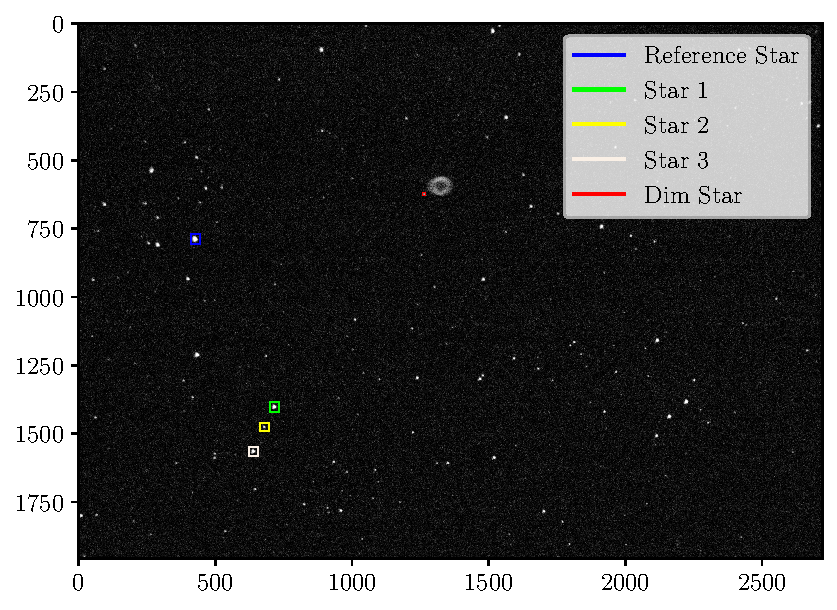
\includegraphics[width=\linewidth]{../fig/crop}
		\caption{نام‌گذاری و کادر ستاره‌ها.}
	\end{figure}
	
	\newgeometry{top=0.2in, bottom=0.2in, left=1in, right=1in}
	\begin{figure}[h!]
		\centering
		\begin{subfigure}{0.49\linewidth}
			\centering
			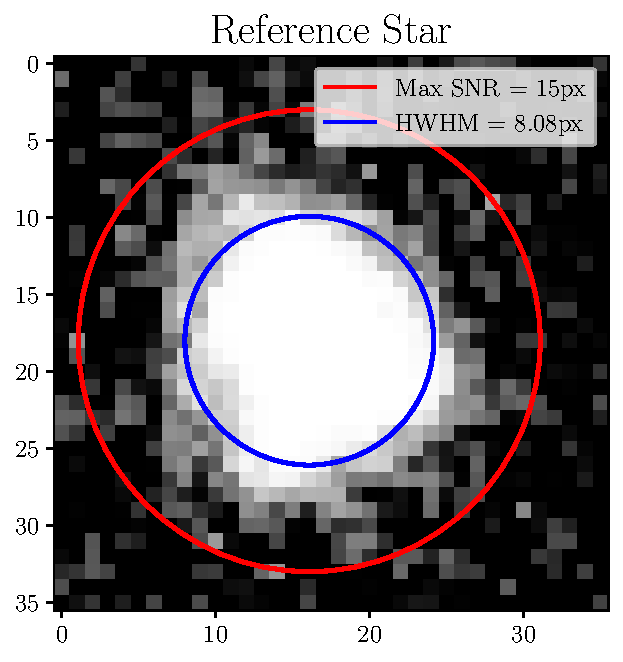
\includegraphics[width=\linewidth]{../fig/reference}
			\caption{ستاره مرجع}
		\end{subfigure}
		\begin{subfigure}{0.49\linewidth}
			\centering
			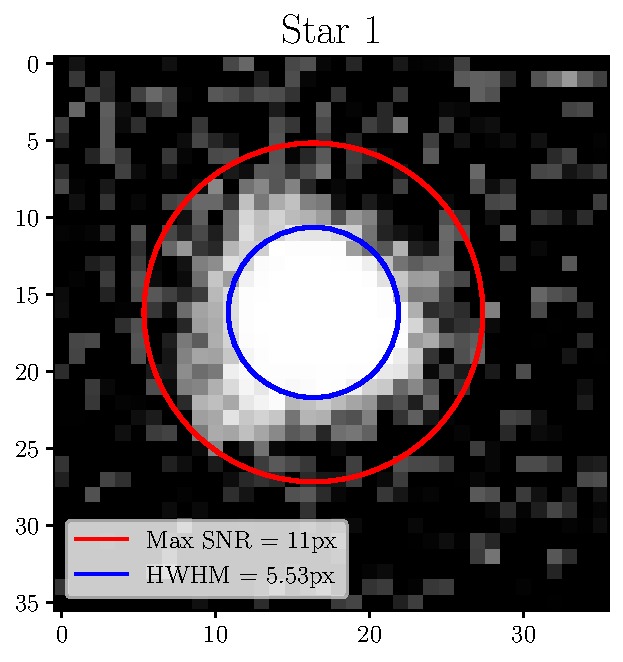
\includegraphics[width=\linewidth]{../fig/star1}
			\caption{ستاره پرنور اول (بالا سمت راست)}
		\end{subfigure}
		\begin{subfigure}{0.49\linewidth}
			\centering
			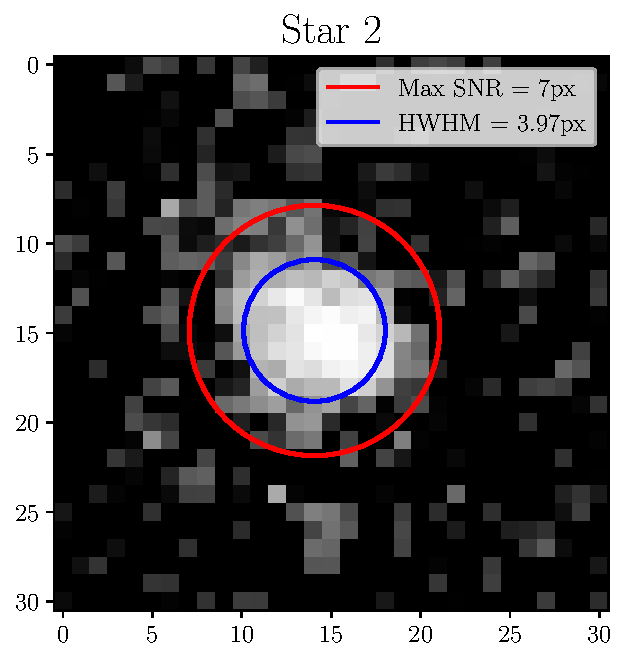
\includegraphics[width=\linewidth]{../fig/star2}
			\caption{ستاره پرنور دوم (وسط)}
		\end{subfigure}
		\begin{subfigure}{0.49\linewidth}
			\centering
			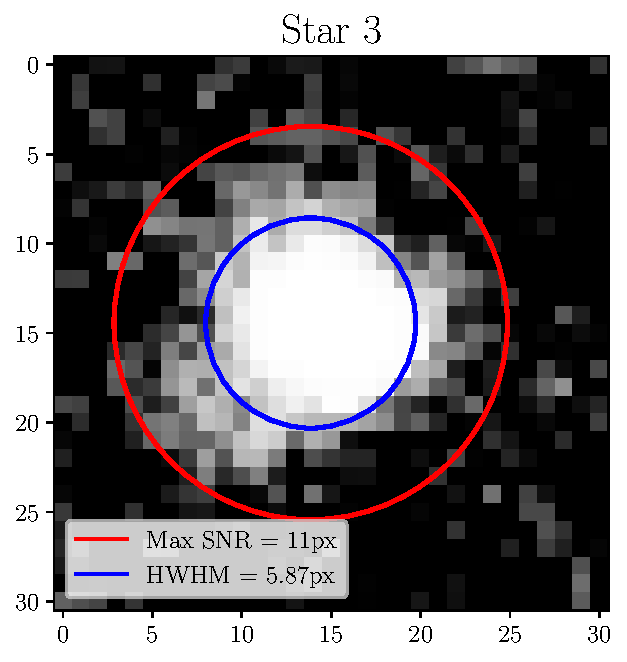
\includegraphics[width=\linewidth]{../fig/star3}
			\caption{ستاره پرنور سوم (پایین سمت راست)}
		\end{subfigure}
		\begin{subfigure}{0.49\linewidth}
			\centering
			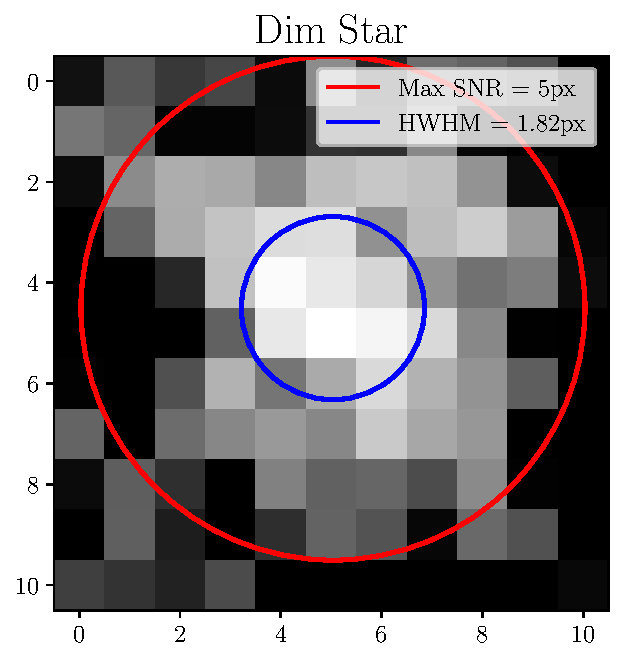
\includegraphics[width=\linewidth]{../fig/dim}
			\caption{ستاره کم‌نور}
		\end{subfigure}
		\caption{مقایسه شعاع ستاره‌ها با دو روش مختلف.}
	\end{figure}
	\restoregeometry
	\section{نتایج}
	\begin{table}[h!]
		\centering
		\caption{قدر هر ستاره با برابر قرار دادن قدر ستاره مرجع با $8.88$.}
		\begin{LTR}
			\begin{tabular}{|O{c}|c|c|}
				\hline
				\lr{Name} & \lr{Max SNR Magnitude} & \lr{HWHM Magnitude} \\ \hline
				\lr{Reference} & $8.88$ & $8.88$ \\ \hline
				\lr{Star 1} & $9.2998\pm0.0002$ & $9.5158\pm0.0002$ \\ \hline
				\lr{Star 2} & $11.0184\pm0.0003$ & $10.5616\pm0.0003$ \\ \hline
				\lr{Star 3} & $9.3287\pm0.0002$ & $9.5532\pm0.0002$ \\ \hline 
				\lr{Dim Star} & $11.2173\pm0.0002$ & $12.2362\pm0.0003$ \\ \hline
			\end{tabular}
		\end{LTR}
	\end{table}
	دقت کنید که خطای قدر ستاره مرجع به خطای قدر هر ستاره با رابطه پخش خطا جمع می‌شود.
	
	به نظر می‌رسد خطای بدست آمده برای قدر بیش از حد کم است. می‌توان این را به در نظر نگرفتن عدم قطعیت خود روش نورسنجی
	دهانه نسبت داد که باید در عدم قطعیت فعلی ضرب شود. اینکه این مقدار دقیقاً چطور محاسبه شود فراتر از این آزمایش است
	و به آن نپرداختیم.
\end{document}